% Section 4.2 (usage scenario: wildfire, time window), rewritten 2026-11-07 on Test4.
% The author's previous draft is .texbuild/section_4_2.before_rewrite.tex.
% Every number comes from ../Test4/ (results/eval/summary.json, results/cost_table.csv,
% results/sieve_cold/*/numbers.json, data/front_sieve_s8.csv); ../Test4/objectives.md
% says what each paragraph is for.
%
% Preview with the real VGTC class (two columns, 9 pt):
%   TEXINPUTS=~/Desktop/unOrg/vis2026/vgtc-conference//: BSTINPUTS=~/Desktop/unOrg/vis2026/vgtc-conference//: \
%     latexmk -pdf -outdir=.texbuild section_4_2.tex
% To move the section into the paper, copy what lies between the "BEGIN SECTION" and
% "END SECTION" markers, the teaser block into the front matter (\teaser{...}), the
% figures from ../Test4/figures/, and refs_cs2.bib's entries into the paper's .bib.
% Labels this section expects from elsewhere (stubbed in the preview only):
% sec:plugin (the ParaView plugin, Section 3), sec:cs3 (Section 4.3).
\documentclass{vgtc}
\usepackage{times}
\renewcommand*\ttdefault{txtt}
\usepackage{mathptmx}
\usepackage{graphicx}
\usepackage{booktabs}
\usepackage{listings}
\usepackage{xcolor}
\vgtcinsertpkg
\graphicspath{{../Test4/figures/}}

% ---- Preview only: the paper's macros ----
\newcommand{\sname}{Sieve}
\newcommand{\Sname}{Sieve}
\newcommand{\code}[1]{\texttt{#1}}
\lstset{basicstyle=\ttfamily\scriptsize, breaklines=true, columns=fullflexible,
        frame=tb, captionpos=b, showstringspaces=false, aboveskip=4pt, belowskip=2pt}
\renewcommand{\lstlistingname}{Listing}
\crefname{listing}{Listing}{Listings}

\title{Section 4.2 preview}
\onlineid{0}
\vgtccategory{System}

\begin{document}



\setcounter{section}{3}
\section{Usage Scenarios}
\setcounter{subsection}{1}

% ===================== BEGIN SECTION (copy into the paper) =====================
\subsection{Wildfire: Choosing the Time Window from an Overview}
\label{sec:cs2}

\begin{figure}[tb]
  \centering
  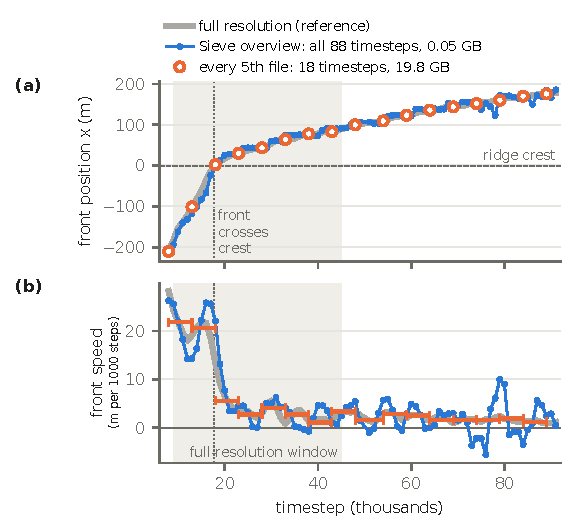
\includegraphics[width=\columnwidth]{fig_cs2_speed}
  \caption{The fire front as each route sees it. (a)~Position. Gray: full resolution at
  every timestep (a reference no route moves). Blue: \sname{}'s overview. Orange rings:
  every fifth file, as a two-pass download's first pass holds them. (b)~Speed: the slope of
  the position over $\pm$2{,}000 steps (gray, blue), and the average between consecutive
  every-fifth files, drawn across the 5{,}000 steps it averages (orange). Shaded: the
  window then fetched at full resolution.}
  \label{fig:cs2speed}
\end{figure}

\begin{figure}[tb]
  \centering
  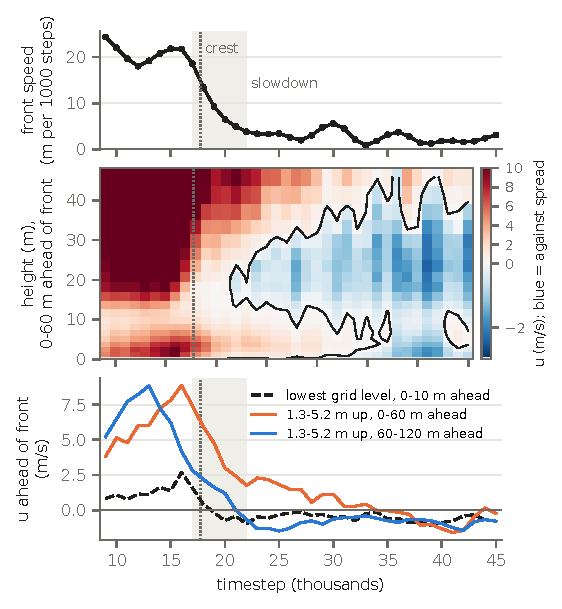
\includegraphics[width=\columnwidth]{fig_cs2_evidence}
  \caption{The answer, from the full-resolution window. All wind values are averaged over
  the burning strip ($|y| \le 50$\,m). (a)~Front speed; shaded: the slowdown. (b)~Wind along
  the spread, $u$, from the front to 60\,m ahead of it, by height and time; blue: against
  the spread; black contour: $u = 0$. (c)~$u$ in the lowest grid level within 10\,m of the
  front (dashed), and at 1.3--5.2\,m within 60\,m (orange) and 60--120\,m ahead
  (blue).}
  \label{fig:cs2evidence}
\end{figure}

\begin{table}[t]
  \centering
  \small
  \setlength{\tabcolsep}{3pt}
  \begin{tabular}{@{}lrrrrrr@{}}
    \toprule
     & \multicolumn{3}{c}{GB over the network} & Bytes & Server & Lines \\
    \cmidrule(lr){2-4}
    Route & overview & box & total & vs \Sname{} & time (s) & of code \\
    \midrule
    \Sname{}                     & 0.05  & 0.36  & 0.40  & 1.0$\times$ & 804 & 9 \\
    Scripts on the server        & 0.05  & 0.35  & 0.40  & 1.0$\times$ & 719 & 111 \\
    Two-pass download$^\dagger$  & 19.76 & 32.94 & 52.70 & 131$\times$ & --- & 99 \\
    Download everything          & 96.62 & 0     & 96.62 & 240$\times$ & --- & 91 \\
    \bottomrule
  \end{tabular}\\[2pt]
  \parbox{\columnwidth}{\footnotesize $^\dagger$Its overview holds 18 timesteps (every
  fifth file); every other route's holds all 88.}\par\vspace{3pt}
  \caption{What each route moves over the network to deliver the same two results: the
  overview, and the window and box at full resolution. \sname{}'s and the scripts' outputs
  are identical, bit for bit. Server time is the time spent on the server reading and
  cutting; reads on the server are examined in \cref{sec:cs3}.}
  \label{tab:cs2}
\end{table}

\begin{table}[t]
  \centering
  \small
  \begin{tabular}{@{}lrr@{}}
    \toprule
    \Sname{} request & Estimated (GB) & Sent (GB) \\
    \midrule
    Overview (all 88 timesteps)  & 0.15 & 0.05 \\
    Box (37 timesteps)           & 0.46 & 0.36 \\
    \bottomrule
  \end{tabular}
  \caption{\sname{}'s estimate of each request, given before anything moves, against what
  it sent. The estimate counts the arrays uncompressed; \sname{} compresses what it sends.
  The box's estimate is sized on the grid positions the overview brought back.}
  \label{tab:cs2est}
\end{table}



\subsubsection{Data and Analysis Requirements}

The dataset is a FIRETEC simulation~\cite{linn2002firetec} of a fire spreading over a
ridge. It is stored on a remote server as 88 VTK files, one per saved timestep, each
1.1\,GB (96.6\,GB in total). Each file holds nine variables on a $600 \times 500 \times 61$
terrain-following grid that lists the position of every grid point. The wind blows across
the ridge and the fire spreads with it: up the windward slope, over the crest at
$x \approx -2$\,m, and down the lee slope. Time is given in simulation steps; the files do
not record the length of a step.

\paragraph{Scientific Task}
In coupled fire--atmosphere simulations, the air just ahead of a fire can reverse and flow
back toward it~\cite{dupuy2011indraft}. Dupuy et al.\ find this \emph{indraft} in the lowest
grid cell, typically within 10\,m of the fire; only when the fire spreads downslope does it
reach farther, up to 30\,m ahead in shrubland and 40\,m in grassland under a weak wind. In this run, the fire slows once it crosses the crest. The
scientist asks whether, as it slows, the wind near the ground ahead of the front reverses
and blows against the spread.

Answering this takes two kinds of data. The first is \emph{when} the fire crosses the crest
and slows. The series must be sampled densely enough to time the drop, and how densely is
not known in advance. The second is the wind in the lowest meters, near the front. An
indraft lives in the lowest grid levels and the first meters ahead of the fire, so this
needs the grid's full resolution, but only around the slowdown and only near the front.

Without \sname{}, the scientist can copy the whole series; download every fifth file to
find the slowdown, then the files of the chosen window; or write scripts that cut both on
the server and copy the cuts back (\cref{tab:cs2}). With \sname{}, the scientist follows
the visual information-seeking mantra, overview first, then zoom, filter, and details on
demand~\cite{shneiderman1996eyes}, across the network and over time. From ParaView,
through \sname{}'s plugin (\cref{sec:plugin}), the scientist
(1)~requests an overview that keeps every timestep at reduced resolution
(\cref{lst:cs2});
(2)~chooses the time window and draws the box on that overview, with nothing moved; and
(3)~requests the window and the box at full resolution (\cref{fig:teaser}).
Each request is priced before anything moves, runs next to the data, and returns only its
result, which ParaView opens in place. The measurements below are from re-running the two
requests, as listed, from an empty cache.

\begin{lstlisting}[language=Python, label=lst:cs2, caption={Step~1: the
overview. Every timestep, every eighth grid point along each axis, five fields.}]
src  = source("ssh://host/wildfire/")  # 88 files
view = fields(src, ["rhof_1", "theta", "u", "v", "w"])
view = subsample(view, 8)
save(view, "overview.vts")
\end{lstlisting}

\subsubsection{Step 1: An Overview of Every Timestep}

The overview keeps every eighth grid point along each axis ($75 \times 63 \times 8$ points
per timestep) and the five fields that follow the fire: the wind (\code{u}, \code{v},
\code{w}), temperature (\code{theta}), and the fuel left (\code{rhof\_1}). \sname{}
returned all 88 timesteps in 47\,MB, 0.05\,\% of the series. Downloading every fifth file
instead moves 19.8\,GB, about 420 times as much, for 18 timesteps.

The overview follows the front through the whole run (\cref{fig:cs2speed}a). Played in
ParaView, it shows the fire slowing once it crosses the ridge. To time this, we ran a
separate script on the overview \sname{} returned: in each timestep it takes the front as
the farthest point downwind where the lowest grid level is at least 400\,K, within 50\,m
of the centreline, and divides the distance the front moves by the steps between
timesteps. The same front can be tracked inside ParaView with its Threshold and Plot Data
Over Time filters; \sname{} supplies the data, not the analysis. On the overview alone, the
front advances at 21\,m per 1{,}000 steps on the windward slope, reaches the
crest between steps 18{,}000 and 19{,}000, and moves at 2.8\,m per 1{,}000 steps on the lee slope; the drop
happens between steps 17{,}000 and 22{,}000. Every fifth file shows the same broad
slowdown, but most of the drop falls inside one of its 5{,}000-step gaps
(\cref{fig:cs2speed}b). Sampling the files risks missing exactly the moment the scientist is
looking for. The overview carries no such risk: it keeps every timestep and thins only the
grid. Without \sname{}, getting it means logging in to the server, writing and running a
script that cuts every file, copying the results back, and loading them into a
visualization tool; with \sname{} it is one four-line request (\cref{lst:cs2}), issued
from ParaView.

\emph{Is the overview enough to find the slowdown?} We compared it with the front computed
at full resolution for every timestep, in a separate evaluation pass on the server. At
every eighth point, the overview finds the fire at all 83 timesteps that have one; its
front lies a median of 4.4\,m from the full-resolution front (within one 16\,m grid spacing
at 92\,\% of timesteps), and it places the crest crossing one timestep (1{,}000 steps)
late. Every fourth point
gains 3\,m of accuracy for eight times the bytes. Every sixteenth point misses the fire at
14 of the 83 timesteps and places the crossing two timesteps late. Every eighth point is
the coarsest overview that still answers \emph{when}.

The overview cannot answer the second question. Below 12\,m above the ground it keeps two
grid levels, the lowest and one at 11.8\,m, of the nine the grid has there. In the lowest
level, from the front to 60\,m ahead of it, the overview's wind turns slightly negative
from step 19{,}000, just after the crest crossing, while the level above stays near zero.
With no levels between the lowest and 11.8\,m, the overview cannot tell whether this
reversal is confined to the lowest level or fills the first meters of air the fire
spreads into.

\subsubsection{Steps 2 and 3: The Window and the Box at Full Resolution}

From the overview, the scientist chose the window from step 9{,}000 to 45{,}000
(37 timesteps): it starts 8{,}000 steps before the drop and runs through the slow lee
phase. On the overview in ParaView, they drew a box over the crest and the lee slope
(\cref{fig:teaser}); the plugin turned it into a \code{region} in the data's own
coordinates. On this terrain-following grid the box holds $151 \times 121 \times 39$
points per timestep, with all nine grid levels below 12\,m. Before fetching, \sname{} estimated
the request's size, using the grid positions the overview had brought back
(\cref{tab:cs2est}); it then returned the 37 timesteps at full resolution in 0.36\,GB. A two-pass download copies the window's files whole: 32.9\,GB.
The overview and the box are both saved with the position of every grid point, so the box sits
inside the overview in ParaView without any alignment step (\cref{fig:teaser}).

\subsubsection{Results}

\Cref{fig:cs2evidence} answers the question. During the slowdown, between steps 17{,}000
and 22{,}000, the front's speed falls from 23 to 4\,m per 1{,}000 steps. Over the same
steps, the air 1.3--5.2\,m above the ground within 60\,m ahead of the front weakens from
+8.9 to +1.8\,m/s, but keeps blowing with the spread until step 34{,}000. Only the lowest
grid level reverses during the slowdown: within 10\,m of the front it is negative from step
19{,}000, while the levels above it still blow forward at 4 to 7\,m/s. This is the shallow
indraft Dupuy et al.\ describe~\cite{dupuy2011indraft}. The overview held that level; only
the full-resolution data shows that the reversal is confined to it.

The reversal of the air the fire spreads into comes later, and farther ahead. At
1.3--5.2\,m and 60--120\,m ahead of the front, the wind stops at step 21{,}000 and reverses
after it; between 13.8 and 18.2\,m above the ground, within 60\,m of the front, it reverses
from step 22{,}000. It is confined to where the fire burns: on the lee slope
($x$ = 100--160\,m, 1.3--5.2\,m up), from step 21{,}000 to 45{,}000, the wind is reversed at
all 25 timesteps inside the burning strip and at none in the flanks ($|y| \ge 90$\,m).

The slowdown thus coincides with the near-ground wind ahead of the front \emph{weakening},
not reversing; the reversal follows, first aloft and farther downslope, and only where the
fire burns. The analysis times the reversal; it does not establish its cause. Before the
fire arrives (steps 2{,}000 to 5{,}000), the near-ground air over the lee slope already
flows against the wind, at 2 to 6\,m/s, in the flanks as much as in the strip, so the
terrain alone can reverse it. The height of the lowest grid level above the ground is not
recorded in the files; the heights above are measured from it.

Every route in \cref{tab:cs2} delivers the same two results. \sname{} and the scripts on
the server move the same 0.40\,GB, and their outputs are identical, bit for bit. The
scripts take 111 lines on two machines: cutting next to the data, copying the cuts back,
and rebuilding the VTK series locally, after logging in to the server. \sname{}'s two
requests take 9 lines, which the plugin writes. On the server, \sname{}'s requests took
804\,s and the scripts 719\,s. The two-pass download moves 131 times \sname{}'s bytes and
sees only 18 timesteps before choosing the window; copying the whole series moves 240
times as much.

The same pattern applies whenever the time of an event in a remote series is unknown: a
storm forming, two structures merging, a flow becoming unstable. An overview that keeps
every timestep, cheap enough to take whole, lets the scientist find the event before
committing to a sampling; a second request then fetches only the moment and the place
that matter, at full resolution.
% ====================== END SECTION (copy into the paper) ======================

% ============ TEASER (front matter in the paper; placed last in this preview) ============
\begin{figure*}[t]
  \centering
  \begin{minipage}[c]{0.56\textwidth}
    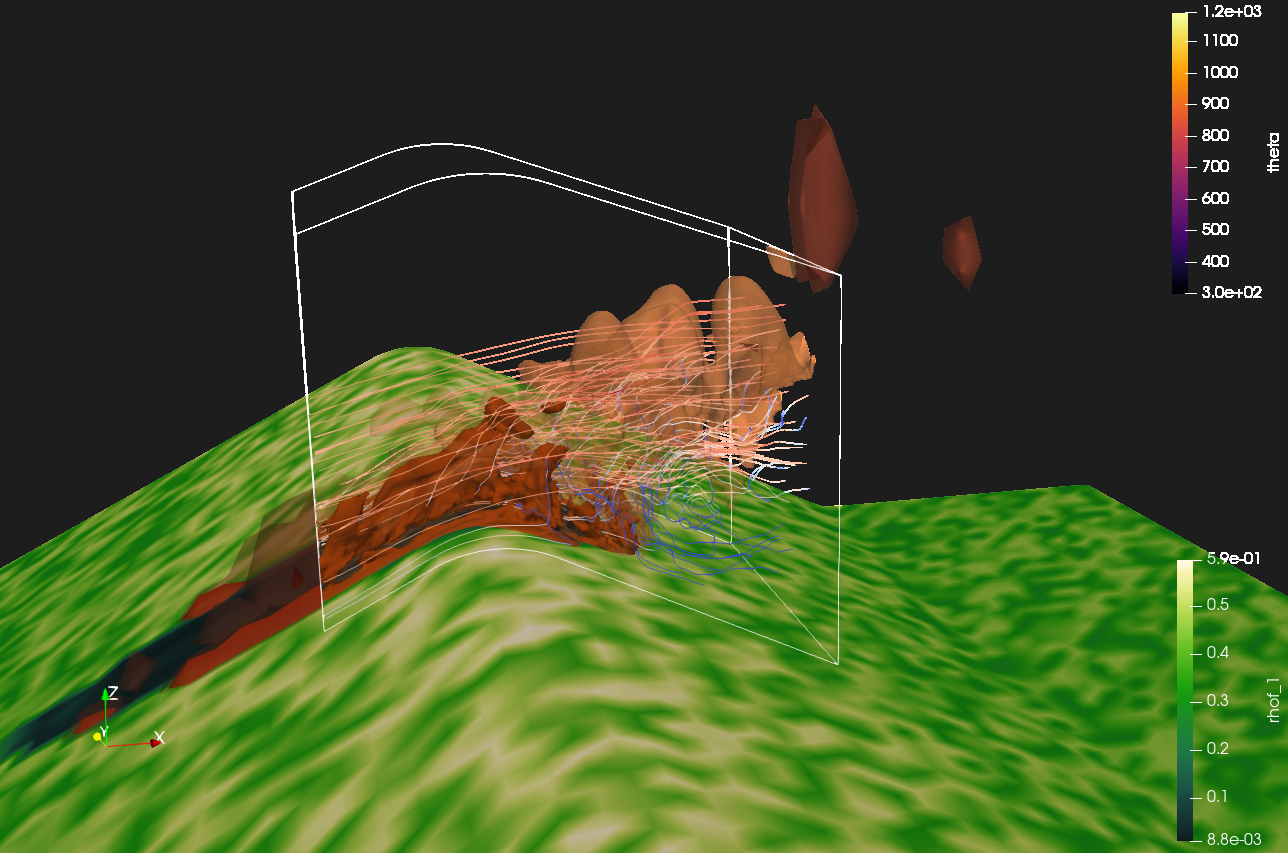
\includegraphics[width=\linewidth]{teaser_paraview}
  \end{minipage}\hfill
  \begin{minipage}[c]{0.42\textwidth}
\begin{lstlisting}[language=Python, numbers=none, frame=tb, aboveskip=0pt, keepspaces=true, basicstyle=\ttfamily\fontsize{8}{9.5}\selectfont]
src  = source("ssh://host/wildfire/")
view = timesteps(src, 9000, 45000)
view = fields(view, ["theta", "u", "v", "w"])
view = region(view, x=(-100, 200), y=(-120, 120),
              z=(0, 350), coords="world")
save(view, "box.vts")
\end{lstlisting}
\vspace{12pt}
\begin{lstlisting}[numbers=none, frame=tb, aboveskip=0pt, keepspaces=true, basicstyle=\ttfamily\fontsize{6.8}{8}\selectfont\color{black!75}]
# from the provenance record in each output
Steps
  1. timesteps  keep timesteps #9000 to #45000
  2. fields     keep theta, u, v, w; drop O2, ...
  3. region     keep the samples inside the box
                (world coordinates), placed on
                the file's geometry
  4. save       write one VTK StructuredGrid file
                per timestep: each point at its
                own position from the source
\end{lstlisting}
  \end{minipage}
  \caption{A fire crossing a ridge, from a 96.6\,GB simulation on a remote server, opened
  in ParaView. Outside the white box: \sname{}'s overview, every timestep at every eighth
  grid point (47\,MB). Inside it: the time window and the region the scientist chose on
  that overview, fetched at full resolution (0.36\,GB) by the request shown (top right).
  \sname{} explains each output in a provenance record (bottom right, excerpt). Both
  outputs carry the positions of their grid points, so ParaView places the detail inside
  the overview with no alignment step. \textbf{[TODO: confirm the rendered timestep and
  the encodings: terrain colored by fuel left, the fire as a temperature surface, lines
  inside the box as streamlines of the full-resolution wind.]}}
  \label{fig:teaser}
\end{figure*}

% ---- Preview only: labels for the sections this one points to (prints nothing) ----
\begingroup
\setcounter{section}{3}\setcounter{subsection}{1}\setcounter{subsubsection}{6}%
\refstepcounter{subsubsection}\label{sec:plugin}%
\setcounter{section}{4}\setcounter{subsection}{2}%
\refstepcounter{subsection}\label{sec:cs3}%
\endgroup

\bibliographystyle{abbrv-doi}
\bibliography{refs_cs2}

\end{document}
